%% LaTeX-Beamer template for KIT design
%% by Erik Burger, Christian Hammer
%% title picture by Klaus Krogmann
%%
%% version 2.1
%%
%% mostly compatible to KIT corporate design v2.0
%% http://intranet.kit.edu/gestaltungsrichtlinien.php
%%
%% Problems, bugs and comments to
%% burger@kit.edu

\documentclass[18pt]{beamer}

%% SLIDE FORMAT

% use 'beamerthemekit' for standard 4:3 ratio
% for widescreen slides (16:9), use 'beamerthemekitwide'

\usepackage{templates/beamerthemekit}
% \usepackage{templates/beamerthemekitwide}

%% TITLE PICTURE

% if a custom picture is to be used on the title page, copy it into the 'logos'
% directory, in the line below, replace 'mypicture' with the 
% filename (without extension) and uncomment the following line
% (picture proportions: 63 : 20 for standard, 169 : 40 for wide
% *.eps format if you use latex+dvips+ps2pdf, 
% *.jpg/*.png/*.pdf if you use pdflatex)

%\titleimage{mypicture}

%% TITLE LOGO

% for a custom logo on the front page, copy your file into the 'logos'
% directory, insert the filename in the line below and uncomment it

%\titlelogo{mylogo}

% (*.eps format if you use latex+dvips+ps2pdf,
% *.jpg/*.png/*.pdf if you use pdflatex)

%% TikZ INTEGRATION

% use these packages for PCM symbols and UML classes
\usepackage{templates/tikzkit}
% \usepackage{templates/tikzuml}

% the presentation starts here

\title[Algorithmische Geometrie]{Algorithmische Geometrie}
\subtitle{ICPC Praktikum 2012}
\author{Huyen Chau Nguyen, Matthias Holoch}

\institute{Institut für Theoretische Informatik}

% Bibliography

\usepackage[citestyle=authoryear,bibstyle=numeric,hyperref,backend=biber]{biblatex}
\addbibresource{templates/example.bib}
\bibhang1em

\begin{document}

% change the following line to "ngerman" for German style date and logos
\selectlanguage{ngerman}

%title page
\begin{frame}
\titlepage
\end{frame}

%table of contents
\begin{frame}{Outline/Gliederung}
\tableofcontents
\end{frame}

% our chapters:
\section{Koordinatenkompression}
\begin{frame}
	\begin{center}
		\textbf{\LARGE{Koordinatenkompression}}
	\end{center}
\end{frame}

\subsection{Was ist das?}
\begin{frame}
	\frametitle{{Koordinatenkompression}}
	\begin{itemize}
		\item Abbilden von gegebenen Koordinaten auf geschicktere Koordinaten
		\pause
		\item Was hei"st geschickt?
		\pause
		\begin{itemize}
			\item Der Algorithmus soll dadurch schneller werden
			\pause
			\item Das Ergebnis darf nicht verfälscht werden
		\end{itemize}
		\pause
		\item Also: Irrelevante Bereiche aussparen
	\end{itemize}
\end{frame}

\subsection{Bei Fl\"achenberechnungen}
\begin{frame}
	\frametitle{{Fl\"achenberechnung}}
	\begin{block}{Das Problem}
	\begin{itemize}
		\pause
		\item{Eingabe:}
		\pause
		\begin{itemize}
			\item Eine 2-dimensionale Figur
			\item Bestehend aus Rechtecken
			\begin{itemize}
				\item Punkt unten links
				\item Punkt oben rechts
				\item Seiten parallel zu den Koordinatenachsen
			\end{itemize}
		\end{itemize}
		\pause
		\item{Ausgabe:}
		\pause
		\begin{itemize}
			\item{Fl\"acheninhalt der Figur}
		\end{itemize}
	\end{itemize}
	\end{block}
\end{frame}
\begin{frame}
	\frametitle{{Fl\"achenberechnung, erster Ansatz}}
	\begin{itemize}
		\item Iteration \"uber alle Datenfelder
		\pause
		\item Aufsummieren aller belegter Datenfelder
	\end{itemize}
\end{frame}
\begin{frame}
	\frametitle{{Fl\"achenberechnung, erster Ansatz}}
	\begin{itemize}
		\item Iteration \"uber alle Datenfelder
		\item Aufsummieren aller belegter Datenfelder
	\end{itemize}
	\begin{figure}
		\begin{center}
			
\includegraphics[scale=0.50]{bilder/kidding.png}		
		\end{center}
	\end{figure}
\end{frame}
\begin{frame}
	\frametitle{{Fl\"achenberechnung mit Koordinatenkompression}}
		\pause
	\begin{itemize}
		\item Vorarbeit
		\pause
		\begin{itemize}
			\item Kompression auf ein Feld maximal der Gr\"o"se $\mathcal (2 \cdot \left|Rechtecke\right|)\times(2 \cdot \left|Rechtecke\right|)$
			\pause
			\item Kleiner, falls sich Rechtecke eine x- oder y-Stelle teilen
			\pause
			\item Merken der tats\"achlichen Gr\"o"se
		\end{itemize}
		\pause
		\item Nun wie gehabt belegte Felder z\"ahlen
			\pause
		\begin{itemize}
			\item dabei deren tats\"achliche Fl\"achen aufsummieren
		\end{itemize}
	\end{itemize}
\end{frame}

\subsection{Weitere Anwendungsgebiete}
\begin{frame}
	\frametitle{{Weitere Anwendungsgebiete von Koordinatenkompression}}
	\begin{itemize}
		\item Volumenberechnung
		\pause
		\item Bereichssuchen
	\end{itemize}
\end{frame}
\section{Sweep}
\begin{frame}
	\begin{center}
		\textbf{Sweep}
	\end{center}
\end{frame}

\subsection{Line Segment Intersection}
\begin{frame}
	\frametitle{{Line Segment Intersection}}
	\begin{block}{Das Problem}
	\begin{itemize}
		\pause
		\item{Eingabe:}
		\pause
		\begin{itemize}
			\item{n Liniensegmente}
		\end{itemize}
		\pause
		\item{Ausgabe:}
		\pause
		\begin{itemize}
			\item{Anzahl der Schnittpunkte}
		\end{itemize}
	\end{itemize}
	\end{block}
\end{frame}
\begin{frame}
	\frametitle{{Line Segment Intersection}}
	\begin{itemize}
		\item \textbf{Anwendungsbeispiel}
		\item Schnitt von Layern bei Kartographie-Software
	\end{itemize}
	\begin{figure}
  		\begin{center}
   			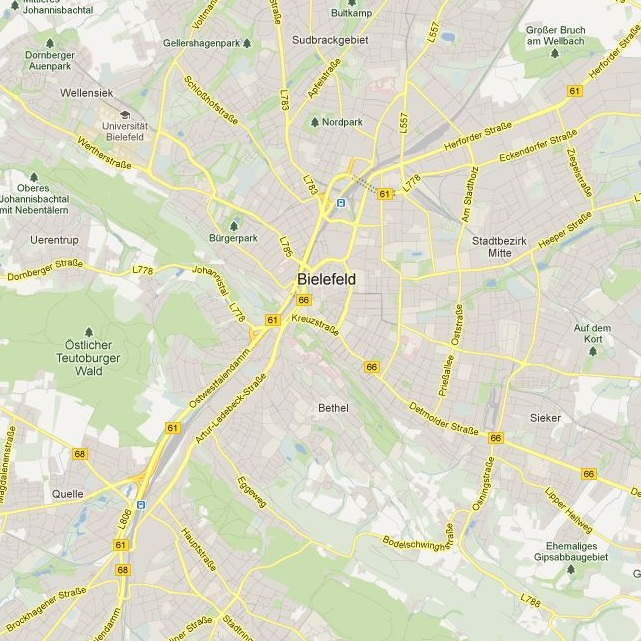
\includegraphics[scale=0.30]{bilder/map.jpg}
 		\end{center}
	\end{figure}
\end{frame}
\begin{frame}
	\frametitle{{Line Segment Intersection}}
	\begin{itemize}
		\item \textbf{Naiv}
		\begin{itemize}
			\pause
			\item{Vergleiche jedes Segment mit jedem anderen}
			\pause
			\item{Resultierende Laufzeit: $\mathcal O(n^2)$}
		\end{itemize}
	\end{itemize}
\end{frame}
\begin{frame}
	\frametitle{{Line Segment Intersection}}
	\begin{itemize}
		\item \textbf{Weitere \"Uberlegungen}
		\pause
		\item{Nur nahe Segmente k\"onnen sich schneiden}
		\pause
		\item{Betrachten der Situation an der Stelle a}
	\end{itemize}
\end{frame}
\begin{frame}
	\frametitle{{Line Segment Intersection}}
	\begin{itemize}
		\item \textbf{Sweep Line Algorithmus, erster Ansatz}
		\pause
	\end{itemize}
	\begin{block}{Ben\"otigte Daten}
		\begin{itemize}
			\item Zustand der Sweep Line S
			\begin{itemize}
				\item Segmente, welche die Sweep Line schneiden
			\end{itemize}
			\pause
			\item Event Queue Q
			\begin{itemize}
				\item Endpunkte der Segmente, aufsteigend geordnet nach ihrer x-Koordinate
			\end{itemize}
		\end{itemize}
	\end{block}
	\begin{itemize}
		\pause
		\item Beginnt ein Segment
		\begin{itemize}
			\pause		
			\item F\"uge das Segment dem Zustand hinzu
			\pause
			\item \"Uberpr\"ufe, ob es Segmente in S schneidet
		\end{itemize}
		\pause
		\item Endet ein Segment
		\begin{itemize}
			\pause
			\item Entferne das Segment aus dem Zustand
		\end{itemize}
		\pause
		\item Das geht noch besser!
	\end{itemize}
\end{frame}
\begin{frame}
	\frametitle{{Line Segment Intersection}}
	\begin{itemize}
		\item \textbf{Sweep Line Algorithmus}
		\pause
		\item Verlgeiche nur direkt benachbarte Segmente
		\pause
		\item Neuer Eventpunkt:
		\begin{itemize}
			\pause
			\item Beim Schnitt zweier Segmente
		\end{itemize}
	\end{itemize}
	\pause
	\begin{block}{Ben\"otigte Daten}
		\begin{itemize}
			\item Zustand der Sweep Line S
			\begin{itemize}
				\item Segmente, welche die Sweep Line schneiden
				\pause
				\item F\"ur jedes Segment die Nachbarn
			\end{itemize}
			\pause
			\item Event Queue Q
			\begin{itemize}
				\item Endpunkte der Segmente
				\pause
				\item Schnittpunkte zwischen Segmenten
			\end{itemize}
		\end{itemize}
	\end{block}
	\pause
	\begin{itemize}
		\item Bentley Ottmann Algorithmus
		\begin{itemize}
			\item Laufzeit $\mathcal O((n+k)\cdot log(n))$
		\end{itemize}
	\end{itemize}
\end{frame}

\subsection{Allgemeine Eigenschaften}
\begin{frame}
	\frametitle{{Allgemeine Eigenschaften von Sweep Algorithmen}}
	\begin{itemize}
		\item Anwendbar auf Probleme beliebig hoher Dimension
		\begin{itemize}
			\pause
			\item{Im 2-Dimensionalen Raum}
			\begin{itemize}
				\item{Gerade, die \"uber sich über die Ebene bewegt}
			\end{itemize}
			\pause
			\item{Im 3-Dimensionalen Raum}
			\begin{itemize}
				\item{Ebene, die sich durch den Raum bewegt}
			\end{itemize}
		\end{itemize}
	\end{itemize}
\end{frame}

\subsection{Weitere Algorithmen}
\begin{frame}
	\frametitle{{Weitere Sweep Algorithmen}}
	\begin{itemize}
		\pause
		\item Fortune's algorithm
		\begin{itemize}
			\item Sweep Line Algorithmus zur Erstellung eines Voronoi-Diagramms
			\pause			
			\item M\"ogliches Anwendungsgebiet: Robotik, Hindernissen fern bleiben
		\end{itemize}
		\pause
		\item Boolsche Operationen auf Polygone
		\begin{itemize}
			\item M\"ogliche Anwendungsgebiete: Computergraphik oder CAD-Systeme
		\end{itemize}
		\pause
		\item Closest Pair
		\pause
		\item Viele mehr!
	\end{itemize}
\end{frame}


\appendix
%\beginbackup

%\begin{frame}[allowframebreaks]{References}
%\printbibliography
%\end{frame}

%\backupend

\end{document}
